
\section{簇的态射纤维的维数}

在本节中，我们将证明：\trVariety{}的\trMorphism{}之\trFiber{}的\trDimension，其表现方式正如你从几何直觉所期待的那样。我们直到此刻才来讨论它的原因是：我们将用到定理~12.2.9（对\trVariety{}而言，\trCodimension{}是\trDimension{}之差）。

在动手之前，先确保我们与直觉处在同一页上。消元理论（定理~8.4.10）告诉我们：投射 $\pi\colon\mathbb{P}^{\mathfrak{n}}_A\to\Spec A$ 是闭的。我们可以这样解读这件事：$\mathbb{P}^{\mathfrak{n}}_A$ 的一个\trClosedSubset{} $X$ 由 $\mathfrak{n}+1$ 个变量的一组齐次方程（在 $A$ 上）切出。$X$ 的\trImage{}就是 $\Spec A$ 中这些方程具有公共非平凡解的那个子集。只要肯下功夫，我们就可以把这件事说成：非平凡解的\emph{存在性}（或者在 $\pi\colon X\to\Spec A$ 之下某点存在原像这件事）是一桩「\trUpperSemicontinuous」的事实。更一般地，你的直觉或许会告诉你：$A$ 上 $\mathfrak{n}+1$ 个变量的一组齐次多项式，其解空间（在 $\mathbb{P}^{\mathfrak{n}}_A$ 中）\trDimension{}至少为 $\mathrm{d}$ 的那个\trLocus，应当是 $\Spec A$ 的一个\trClosedSubset。（作为一个特例，考虑线性方程：$\mathfrak{n}+1$ 个变量的 $\mathfrak{m}$ 个线性方程具有\trDimension{}至少为 $\mathrm{d}+1$ 的解空间，这一条件是系数上的一个闭条件——你能借助线性代数看出为什么吗？）这个直觉将是正确的，而且将以一种根本的方式用到\trProperness（定理~12.4.3(b)）。我们还将阐明\emph{源}上\trFiber\trDimension{}的\trUpperSemicontinuous{}性（定理~12.4.3(a)）。一个值得想透的有用例子是从 $xy$-平面到 $xz$-平面的\trMap（$\Spec k[x,y]\to\Spec k[x,z]$），由 $(x,z)\mapsto(x,xy)$ 给出。（这个例子也曾在 \S8.4.1 中出现过。）

我们实质性的讨论，从一条在\trLocally\trNoetherian{}设定下更一般地成立的不等式开始。

\textbf{12.4.A.（关键练习：\trCodimension{}对\trMorphism{}的表现正如你所期待，或「\trFiber\trDimension{}绝不会低于预期」）}\quad 设 $\pi\colon X\to Y$ 是\trLocally\trNoetherian{}\trScheme{}之间的一个\trMorphism，而 $\mathfrak{p}\in X$ 与 $\mathfrak{q}\in Y$ 是满足 $\mathfrak{q}=\pi(\mathfrak{p})$ 的两点。证明：
\[
\operatorname{codim}_X\mathfrak{p}\le\operatorname{codim}_Y\mathfrak{q}+\operatorname{codim}_{\pi^{-1}(\mathfrak{q})}\mathfrak{p}
\]
（见\cref{fig:codim-fiber-inequality}）。（这与\mbox{练习~12.1.K}相似，但它并不相同！）提示：取 $\mathfrak{q}$「在 $Y$ 中」的一组\trSystemOfParameters（定义~12.3.11），再取 $\mathfrak{p}$「在 $\pi^{-1}(\mathfrak{q})$ 中」的一组\trSystemOfParameters，并用它们找出 $\OO_{X,\mathfrak{p}}$ 的 $\operatorname{codim}_Y\mathfrak{q}+\operatorname{codim}_{\pi^{-1}(\mathfrak{q})}\mathfrak{p}$ 个元素，使它们在 $\Spec\OO_{X,\mathfrak{p}}$ 中切出 $\mathfrak{p}=[\mathfrak{m}]$。用\mbox{练习~12.3.K}。

\begin{figure}[htbp]
\centering
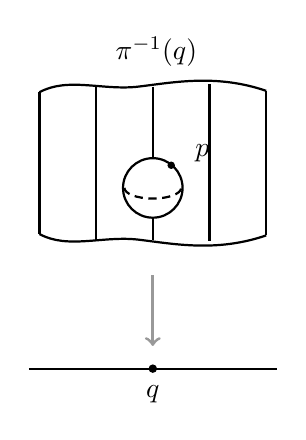
\begin{tikzpicture}[scale=0.9,line width=0.8pt]
  \draw (-1.6,1.0) .. controls (-1.2,1.22) and (-0.7,1.02) .. (-0.2,1.08)
        .. controls (0.3,1.14) and (0.9,1.26) .. (1.6,1.02);
  \draw (-1.6,-1.0) .. controls (-1.2,-1.22) and (-0.7,-1.02) .. (-0.2,-1.08)
        .. controls (0.3,-1.14) and (0.9,-1.26) .. (1.6,-1.02);
  \draw (-1.6,1.0) -- (-1.6,-1.0);
  \draw (1.6,1.02) -- (1.6,-1.02);
  \draw (-0.8,1.10) -- (-0.8,-1.08);
  \draw (0.8,1.12) -- (0.8,-1.10);
  \draw (0,1.08) -- (0,-1.08);
  \filldraw[fill=white] (0,-0.35) circle (0.42);
  \draw[densely dashed] (-0.40,-0.35) arc[start angle=180, end angle=360, x radius=0.40, y radius=0.15];
  \fill (0.26,-0.03) circle (1.5pt);
  \node at (0.70,0.14) {$\mathfrak{p}$};
  \node[anchor=south] at (0.05,1.22) {$\pi^{-1}(\mathfrak{q})$};
  \draw[gray!80,line width=1.1pt,->] (0,-1.58) -- (0,-2.58);
  \draw (-1.75,-2.90) -- (1.75,-2.90);
  \fill (0,-2.90) circle (1.7pt);
  \node at (0,-3.26) {$\mathfrak{q}$};
\end{tikzpicture}
\caption{\mbox{练习~12.4.A}：全空间中一点的\trCodimension，被「该点在\trFiber{}中的\trCodimension」与「其\trImage{}在靶中的\trCodimension」之和所界。（依原书手绘图重绘。）}\label{fig:codim-fiber-inequality}
\end{figure}

\mbox{练习~12.4.A}与你的几何直觉相合吗？你应当能举出一些富有启发性的例子：既有等号成立的，也有等号失败的。我们将看到：对足够好的——即\trFlat{}的——\trMorphism，等号总成立；见命题~24.5.6。

现在我们来证明：\mbox{练习~12.4.A}的不等式在「$Y$ 的大部分」之上其实取等号。

\textbf{12.4.1.\ \trhTheorem。}\ ——\ \emph{设 $\pi\colon X\to Y$ 是\trIntegral{}\trScheme{}之间的一个\trFiniteType{}\trDominant{}\trMorphism，使得有限生成的\trFieldExtension{} $K(X)/K(Y)$ 具有\trTrDeg{} $\mathfrak{r}$。那么存在一个非空\trOpenSubset{} $\mathsf{U}\subset Y$，使得对一切 $\mathfrak{q}\in\mathsf{U}$，$\mathfrak{q}$ 之上的\trFiber{}非空，且具有\trPureDimension{} $\mathfrak{r}$。}

一个有趣的事实：我们将在证明中使用\trNoetherNormalization{}引理~12.2.4，尽管这条陈述并不涉及\trVariety！如果这条陈述的如此一般性让你介意，我们为\trVariety{}准备了下面的特例。

\textbf{12.4.2.\ \trhCorollary。}\ ——\ \emph{设 $\pi\colon X\to Y$ 是不可约 $k$-\trVariety{}之间的一个（必然\trFiniteType{}的）\trMorphism，$\dim X=\mathfrak{m}$ 而 $\dim Y=\mathfrak{n}$。那么存在一个非空\trOpenSubset{} $\mathsf{U}\subset Y$，使得对一切 $\mathfrak{q}\in\mathsf{U}$，$\mathfrak{q}$ 之上的\trFiber{}具有\trPureDimension{} $\mathfrak{m}-\mathfrak{n}$，或者为空。}

（按约定，空集严格按字面也具有\trPureDimension{} $\mathfrak{r}$——空集的每个\trIrreducibleComponent{}都具有\trDimension{} $\mathfrak{r}$。这使推论~12.4.2 的陈述干净了一点。）

\textbf{12.4.B.（练习）}\quad 验证：定理~12.4.1 蕴涵推论~12.4.2。

\emph{\trhTheorem{}~12.4.1 之证明。}\quad 我们从两个快速的化归开始。(i) 必要时缩小 $Y$，便可设 $Y$ 仿射，比如说 $\Spec B$。(ii) 同样还可设 $X$ 仿射，比如说 $\Spec A$。（理由：以有限多个\trAffine\trOpenSubset{} $X_1,\dots,X_a$ \trCover{} $X$，再对每个 $\pi|_{X_i}$ 取相应诸 $\mathsf{U}$ 的交。）

为了给论证的其余部分提供动机，我们先来描述目标。我们将造出 $\Spec B$ 的一个非空\trDistinguishedOpen{} $\mathsf{U}$，使得 $\pi^{-1}(\mathsf{U})\to\mathsf{U}$ 穿过 $\mathbb{A}^{\mathfrak{r}}_{\mathsf{U}}$ 分解，且所经的是一个有限满\trMorphism：
\begin{equation*}\tag{12.4.2.1}\label{eq:finite-surjective-factorization}
\begin{tikzcd}[row sep=2.6em, column sep=4.4em]
X=\Spec A & \pi^{-1}(\mathsf{U}) \ar[l, hook, "\text{开嵌入}"'] \ar[d, "\text{有限满}"] \\
 & \mathbb{A}^{\mathfrak{r}}_{\mathsf{U}} \ar[d] \\
Y=\Spec B \ar[uu, "\pi"] & \mathsf{U}. \ar[l, hook, "\text{开嵌入}"']
\end{tikzcd}
\end{equation*}

\textbf{12.4.C.（练习）}\quad 证明：这就足以证明定理~12.4.1。提示：设 $\mathfrak{p}\in\mathsf{U}$ 是一点，其\trResidueField{}为 $\kappa$。证明：任何有限地映到 $\mathbb{A}^{\mathfrak{r}}_{\kappa}$ 的不可约\trVariety{}都有至多为 $\mathfrak{r}$ 的\trDimension。这将表明 $\pi^{-1}(\mathfrak{p})$ 的任何分量的\trDimension{}至多为 $\mathfrak{r}$。为了证明等号，对 $\Spec A\to\Spec B[x_1,\dots,x_{\mathfrak{r}}]$ 恰当地应用 Going-Down 定理~12.2.12。

于是，我们现在就来着手搭建交换图~\eqref{eq:finite-surjective-factorization}。我们首先注意到：$B$ 含入 $A$ 与 $K(B)$ 二者，而 $A$ 与 $K(B)$ 又都含入 $K(A)$。从 $A$ 与 $K(B)$ 到 $K(A)$ 的这两个映射都穿过 $A\otimes_B K(B)$ 分解（它的 $\Spec$ 就是 $\pi$ 的\trGenericFiber），故从 $A$ 与 $K(B)$ 到 $A\otimes_B K(B)$ 的映射必为包含。
\begin{equation*}\tag{12.4.2.2}\label{eq:generic-fiber-inclusions}
\begin{tikzcd}[row sep=2.6em, column sep=3.8em]
 & & K(A) \\
A \ar[urr, bend left=8] \ar[rr, hook, "\therefore\hookrightarrow"'] & & A\otimes_B K(B) \ar[u] \\
B \ar[u, hook] \ar[rr, hook] & & K(B) \ar[u, hook, "\therefore\hookrightarrow"] \ar[uu, bend right=32]
\end{tikzcd}
\end{equation*}

显然，$K(A)\otimes_B K(B)=K(A)$（因为 $A\otimes_B K(B)$ 可以解读为：取 $A$，并把其中身为 $B$ 的非零元的那些元素全部可逆化），而 $A\otimes_B K(B)$ 是域 $K(B)$ 上\trFinitelyGenerated{}的一个\trAlgebra。

由\trNoetherNormalization~12.2.4，我们可以找到元素 $t_1,\dots,t_{\mathfrak{r}}\in A\otimes_B K(B)$，它们在 $K(B)$ 上\trAlgebraicallyIndependent，使得 $A\otimes_B K(B)$ 在 $K(B)[t_1,\dots,t_{\mathfrak{r}}]$ 上整。

现在，我们可以把诸元素 $t_i\in A\otimes_B K(B)$ 想成分数：分子在 $A$ 中，分母在 $B$ 中（并且非零）。设 $f$ 是各个 $t_i$ 所出现的那些分母之积，那么把 $B$ 换成 $B_f$（即把 $\Spec B$ 换成它的\trDistinguishedOpen{} $D(f)$）之后，便可设诸 $t_i$ 全都落在 $A$ 中。于是（在草率地把 $B_f$ 重命名为 $B$、把 $A_f$ 重命名为 $A$ 之后），我们可以把交换图~\eqref{eq:generic-fiber-inclusions} 修剪并扩充成下面的样子。
\[
\begin{tikzcd}[row sep=2.6em, column sep=4.2em]
A \ar[r, hook] & A\otimes_B K(B) \\
B[t_1,\dots,t_{\mathfrak{r}}] \ar[u, hook] \ar[r, hook] & K(B)[t_1,\dots,t_{\mathfrak{r}}] \ar[u, hook, "\text{整}"'] \\
B \ar[u, hook] \ar[r, hook] & K(B)
\end{tikzcd}
\]

现在 $A$ 在 $B$ 上\trFinitelyGenerated，从而在 $B[t_1,\dots,t_{\mathfrak{r}}]$ 上也\trFinitelyGenerated。然而我们还不能确信 $A$ 在 $B[t_1,\dots,t_{\mathfrak{r}}]$ 上\emph{\trFinite}，所以事情尚未了结。我们将不得不进一步对 $B$ 取\trLocalization。

设 $A$ 在 $B$ 上由 $u_1,\dots,u_{\mathfrak{q}}$ 生成\footnote{原书以记号 $\mathfrak{q}$ 计生成元个数（又如 $F_{\mathfrak{n}}$、$\mathbb{P}^{\mathfrak{n}}_A$ 以维数 $\mathfrak{n}$ 计仿射片数），与全书惯用斜体下标之例不合，兹照录原书。——译者注}。我们的\trNoetherNormalization{}论证蕴涵：每个 $u_i$ 都满足某个首一方程 $f_i(u_i)=0$，其中 $f_i\in K(B)[t_1,\dots,t_{\mathfrak{r}}][t]$（即：把 $f_i$ 视作 $t$ 的、系数取自 $K(B)[t_1,\dots,t_{\mathfrak{r}}]$ 的多项式时，它是首一的）。诸 $f_i$ 的系数（视作 $t_1,\dots,t_{\mathfrak{r}}$ 与 $t$ 的多项式时）先验地是 $B$ 中的分式，但只要乘上全部那些分母，便可设每个 $f_i\in B[t_1,\dots,t_{\mathfrak{r}}][t]$，代价是丧失诸 $f_i$ 的首一性（这一次是视作 $t$ 的多项式而言）。令 $b\in B$ 为诸 $f_i$ 的首项系数（视作 $t$ 的多项式时）之积。若 $\mathsf{U}=D(b)$（即 $b$ 可逆的那个\trLocus），则在 $\mathsf{U}$ 之上，诸 $f_i$（可以取成）具有首项系数 $1$，于是诸 $u_i$（作为 $A_b$ 中的元素）在 $B_b[t_1,\dots,t_{\mathfrak{r}}]$ 上整。从而 $\Spec A_b\to\Spec B_b[t_1,\dots,t_r]$ 既\trFinite{}又满（后者由 Lying Over 定理~8.2.5）。

至此，我们已如所需造出交换图~\eqref{eq:finite-surjective-factorization}。\hfill$\square$

关于这个证明，有几点值得指出。首先，这条结果最初的动机虽然来自域 $k$ 上的经典\trVariety，证明却用到了\emph{另一个}域——\trFunctionField{} $K(B)$——之上的\trVariety{}论。这正是一个例证，说明把\trGenericPoint{}引进\trAlgebraicGeometry{}大有用处，即便在考虑更「经典」的问题时也是如此。

其次，论证主体部分的想法是：我们在\trGenericPoint{}处有一条结果（$\Spec A\otimes_B K(B)$ 在 $K(B)$ 上的仿射空间之上既\trFinite{}又满），而我们想把它「铺展」到 $\Spec B$ 的\trGenericPoint{}的一个\trOpen\trNeighborhood{}上去。我们的做法是：注意到只要把问题正确地描述出来，就会出现「有限多个分母」，然后把这些分母可逆化。这种「铺展」的想法是一个反复出现的主题。

\textbf{12.4.D.（练习：不可约性的有用判别法）}\quad 设 $\pi\colon X\to Y$ 是到一个不可约\trVariety{}上的一个\trProper{}\trMorphism，而 $\pi$ 的全部\trFiber{}都非空，且都不可约并具有相同的\trDimension。证明：$X$ 不可约。

\textbf{12.4.3.\ \trhTheorem{}（\trFiber\trDimension{}的\trUpperSemicontinuous{}性）。}\ ——\ \emph{设 $\pi\colon X\to Y$ 是\trFiniteType{} $k$-\trScheme{}之间的一个\trMorphism。}
\begin{enumerate}[label=(\alph*)]
\item （\emph{源上的\trUpperSemicontinuous{}性}）$\pi$ 在 $\mathfrak{p}\in X$ 处的\trFiber{}的\trDimension{}（即 $\pi^{-1}(\pi(\mathfrak{p}))$ 中含有 $\mathfrak{p}$ 的那个最大分量的\trDimension）作为 $\mathfrak{p}$ 的函数（也就是说，在 $X$ 上）是\trUpperSemicontinuous{}的。
\item （\emph{靶上的\trUpperSemicontinuous{}性}）再者，若 $\pi$ 还是闭的（例如 $\pi$ \trProper），则 $\pi$ 在 $\mathfrak{q}\in Y$ 之上的\trFiber{}的\trDimension{}作为 $\mathfrak{q}$ 的函数（也就是说，在 $Y$ 上）是\trUpperSemicontinuous{}的。
\end{enumerate}
若把闭性假设去掉，你应当能够立刻为 (b) 构造出一个反例。（我们还提一句：对射影\trMorphism{}而言，定理~12.4.3(b) 已在\mbox{练习~18.1.B}中以简单的方式完成了。）

\emph{证明。}\ (a) 令 $F_{\mathfrak{n}}$ 为 $X$ 的由\trFiber\trDimension{}至少为 $\mathfrak{n}$ 的点组成的子集。我们希望证明：对一切 $\mathfrak{n}$，$F_{\mathfrak{n}}$ 都是\trClosedSubset。我们对 $\dim Y$ 作归纳。基底情形 $\dim Y=0$ 是平凡的。于是固定 $Y$，并假设结果对所有维数更小的靶已知。

\textbf{12.4.E.（练习）}\quad 证明：只需在 $X$ 与 $Y$ 都\trIntegral、且 $\pi$ \trDominant{}的情形下证明这条结果。

令 $\mathfrak{r}=\dim X-\dim Y$ 为 $\pi$ 的「相对维数」。若 $\mathfrak{n}\le\mathfrak{r}$，则由\mbox{练习~12.4.A}（再结合定理~12.2.9，即对\trVariety{}而言\trCodimension{}是\trDimension{}之差），有 $F_{\mathfrak{n}}=X$。

若 $\mathfrak{n}>\mathfrak{r}$，则令 $\mathsf{U}\subset Y$ 为定理~12.4.1 中那个「\trFiber\trDimension{}恰为 $\mathfrak{r}$」的\trDense\trOpenSubset。那么 $F_{\mathfrak{n}}$ 与 $\mathsf{U}$ 的原像不相交。把 $Y$ 换成 $Y\setminus\mathsf{U}$（并把 $X$ 换成 $X\setminus\pi^{-1}(\mathsf{U})$）之后，由归纳假设便告完成。

\textbf{12.4.F.（容易的练习）}\quad 证明 (b)（利用 (a)）。\hfill$\square$

\textbf{12.4.4.\ \trhProposition{}（「\trGenericallyFinite{}蕴涵泛有限」；参看\mbox{练习~10.3.G}）。}\ ——\ \emph{设 $\pi\colon X\to Y$ 是\trDimension{}为 $\mathfrak{n}$ 的不可约 $k$-\trVariety{}之间的一个\trGenericallyFinite{}\trMorphism。那么存在一个\trDense\trOpenSubset{} $\mathsf{V}\subset Y$，使 $\pi$ 在其上\trFinite。}

（如果你愿意，日后可以把不可约性假设放宽为只要求 $X$ 与 $Y$ 具有\trPureDimension{} $\mathfrak{n}$。）

\emph{证明。}\ 如同定理~12.4.1 的证明，我们可以设 $Y$ 仿射，且 $\pi$ \trDominant。设 $X=\bigcup_{i=1}^{\mathfrak{n}}\mathsf{U}_i$\footnote{原书此处上标用维数记号 $\mathfrak{n}$ 计仿射片个数，兹照录原书。——译者注}，其中诸 $\mathsf{U}_i$ 是 $X$ 的\trAffine\trOpenSubscheme。由\mbox{练习~10.3.G}，存在\trDense\trOpenSubset{} $\mathsf{V}_i\subset Y$，使得 $\pi|_{\mathsf{U}_i}$ 在其上\trFinite。把 $Y$ 换成 $\bigcap_i\mathsf{V}_i$ 的一个仿射开子集之后，便可设诸 $\pi|_{\mathsf{U}_i}$ 都\trFinite。

\textbf{12.4.G.（练习）}\quad 证明：$\pi$ 是闭的。提示：你只需要用到 $\pi|_{\mathsf{U}_i}$ 是闭的，以及 $\mathsf{U}_i$ 只有有限多个。

于是 $X\setminus\mathsf{U}_1$ 是一个\trClosedSubset，从而 $\pi(X\setminus\mathsf{U}_1)$ 是闭的。

\textbf{12.4.H.（练习）}\quad 证明：这个闭子集并非整个 $Y$。

令 $\mathsf{V}:=Y\setminus\pi(X\setminus\mathsf{U}_1)$。那么 $\pi$ 在 $\mathsf{V}$ 之上\trFinite：它是把有限\trMorphism{} $\pi|_{\mathsf{U}_1}\colon\mathsf{U}_1\to Y$ 限制到靶 $Y$ 的\trOpenSubset{} $\mathsf{V}$ 上所得的\trMorphism。\hfill$\square$
